\scanpage{5}
\mspage{3}
\deleted{the $\pi_i$ \unsure{of} degree zero}, and \deleted{that} we shall want that
\figure{\begin{tikzpicture}[x=1cm,y=1cm]
\node[anchor=west] at (.8,.55) {$\pi_i=0\quad\text{if }i\notin[0,2n]$};
\node[anchor=west] at (6.9,.55) {fixed \inserted{(even)} interval.};
\node[anchor=east] at (.15,-.7) {$(3.0)$};
\draw (.45,.25)--(.7,.25)--(.65,1.05) .. controls (2,1.2) and (5.4,1.55) .. (6.35,1.4) .. controls (6.65,1.36) and (6.55,.7) .. (6.45,.42)--(6.95,.42);
\draw (.7,0)--(-.1,-.55);
\end{tikzpicture}}
\deleted{Supp} We are concerned here with \uline{uniqueness}. \deleted{Suppose, uniqueness established}

Let us first note that
\[
\mathcal E^0\ni u\quad\Longleftrightarrow\quad(u\pi_i=\pi_i u\quad\forall i)
\]
thus $\mathcal E^0$ is the commutant of the $k$-algebra generated by the $\pi_i$. Thus the $\pi_i$ are in the centre $\mathfrak Z(\mathcal E^0)$ of $\mathcal E^0$, and they are \inserted{\figure{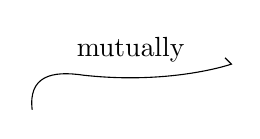
\begin{tikzpicture}[x=1cm,y=1cm,baseline=(reading.base)]\node (reading) at (0,.35) {mutually};\draw (-1.25,-.42) .. controls (-1.3,.01) and (-1,.08) .. (-.6,.02) .. controls (.3,-.08) and (1,.07) .. (1.28,.16)--(1.2,.24);\end{tikzpicture}}} orthogonal projectors with sum $1$ in this commutative ring. Suppose the $\pi_\alpha$ already determined for $\alpha\notin[i,2n-i]$, \inserted{\figure{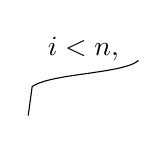
\begin{tikzpicture}[x=1cm,y=1cm,baseline=(reading.base)]\node (reading) at (0,.35) {$i<n$,};\draw (-.7,-.5)--(-.65,-.13) .. controls (-.4,.04) and (.5,.03) .. (.7,.2);\end{tikzpicture}}} and let us determine $\pi_i$ and $\pi_{2n-i}$ [i.e. $\pi_\alpha$ for $\alpha\notin[i+1,2n-i-1]$.]
\inserted{\figure{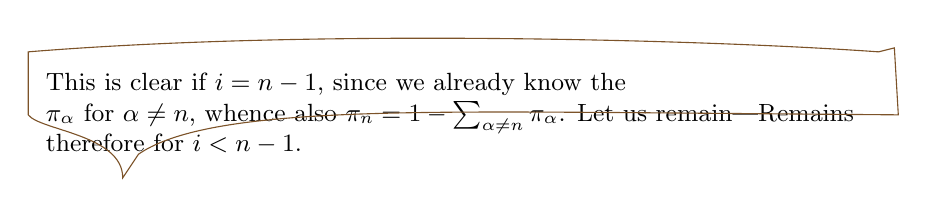
\begin{tikzpicture}[x=1cm,y=1cm]
\node[anchor=north west,align=left,font=\small] at (.2,.8) {This is clear if $i=n-1$, since we already know the\\$\pi_\alpha$ for $\alpha\neq n$, whence also $\pi_n=1-\sum_{\alpha\neq n}\pi_\alpha$. \unsure{Let us remain|Remains}\\therefore for $i<n-1$.};
\draw[draw=brown!65!black] (.1,.95) .. controls (3.8,1.25) and (8.8,1.1) .. (10.9,.95) --(11.1,1.0)--(11.15,.15)--(7.5,.18) .. controls (4.5,.2) and (2.3,.2) .. (1.5,-.35) --(1.3,-.65) .. controls (1.3,-.1) and (.25,-.05) .. (.1,.15)--cycle;
\end{tikzpicture}}}
We therefore know
\[
\varphi_i=\deleted{\unsure{1-\sum\pi_\alpha}}\left(1-\sum_{\alpha<i}\pi_i\right)=\sum_{\alpha\geq i}\pi_\alpha,
\quad\text{and}\quad
\psi_{2n-i}=\left(1-\sum_{\alpha>2n-i}\pi_i\right)=\sum_{\alpha\leq 2n-i}\pi_\alpha
\]
thus also the component
\[
\unsure{or|Now}\quad\psi_{2n-i}\deleted{\unsure{\varphi}}\mathcal E^{2n-2i}\varphi_i
=\sum_\alpha\psi_{2n-i}\pi_{\alpha+(2n-2i)}\mathcal E\pi_\alpha\varphi_i)
\]
Now
\[
\pi_\alpha\varphi_i=\begin{cases}0&\text{if }\alpha<i\\\pi_\alpha&\text{if }\alpha\geq i\end{cases}
\quad\text{and}\quad
\psi_{2n-i}\pi_{\alpha+(2n-2i)}=
\begin{cases}
0&\text{if }\inserted{\text{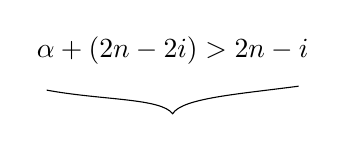
\begin{tikzpicture}[x=1cm,y=1cm,baseline=(reading.base)]\node (reading) at (0,.35) {$\alpha+(2n-2i)>2n-i$};\draw (-1.6,-.15) .. controls (-.9,-.28) and (-.15,-.25) .. (0,-.45) .. controls (.12,-.25) and (.85,-.2) .. (1.6,-.1);\end{tikzpicture}}}\quad\text{i.e. }\alpha>i\\
\pi_{\alpha+(2n-2i)}&\text{if }\inserted{\text{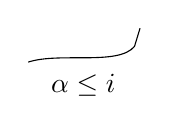
\begin{tikzpicture}[x=1cm,y=1cm,baseline=(reading.base)]\node (reading) at (0,.35) {$\alpha\leq i$};\draw (-.7,.65) .. controls (-.3,.78) and (.45,.6) .. (.65,.85)--(.72,1.08);\end{tikzpicture}}}
\end{cases}
\]
thus the term with index $\alpha$ in the sum $\sum$ is zero unless $\alpha=i$, in which case it is equal to
\[
\pi_{i+(2n-2i)}\mathcal E\pi_i=\pi_{2n-i}\mathcal E\pi_i=\mathcal E_{2n-i,i}.
\]
Thus knowledge of the $\pi_\alpha$ for $\alpha\notin[i,2n-i]$ implies knowledge of $\mathcal E_{\deleted{\unsure{i,2n-i}}\inserted{2n-i,i}}$ \deleted{\unsure{Considered|Considé}}

The condition which will imply uniqueness \deleted{\illegible{1}} of $u_i$,
\mspage{4}
